\begin{figure}[!ht]
\centering
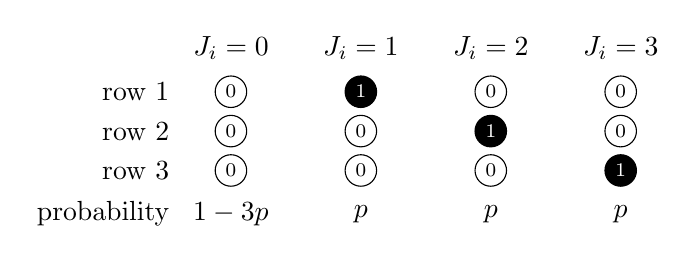
\begin{tikzpicture}[x=1.65cm,y=0.5cm,
  bit/.style={circle,draw,minimum size=4mm,inner sep=0pt},
  present/.style={bit,fill=black,text=white}]
  \foreach \x/\y in {0/1,0/2,0/3,1/1,1/2,2/1,2/3,3/2,3/3}
    \node[bit] at (\x,\y) {\scriptsize 0};
  \foreach \x/\y in {1/3,2/2,3/1}
    \node[present] at (\x,\y) {\scriptsize 1};
  \node at (0,4.1) {$J_i=0$};
  \node at (1,4.1) {$J_i=1$};
  \node at (2,4.1) {$J_i=2$};
  \node at (3,4.1) {$J_i=3$};
  \node at (0,-0.1) {$1-3p$};
  \foreach \x in {1,2,3} {\node at (\x,-0.1) {$p$};}
  \node[anchor=east] at (-0.4,3) {row 1};
  \node[anchor=east] at (-0.4,2) {row 2};
  \node[anchor=east] at (-0.4,1) {row 3};
  \node[anchor=east] at (-0.4,-0.1) {probability};
\end{tikzpicture}
\caption{One coordinate of the sparse coupling, illustrated with three
rows and $3p<1$. Each row contains this coordinate with probability $p$;
the union contains it with probability $3p$. Making these choices
independently across coordinates gives the required product laws.}
\label{fig:coupling}
\end{figure}
